\begin{figure}[t]
    \centering
    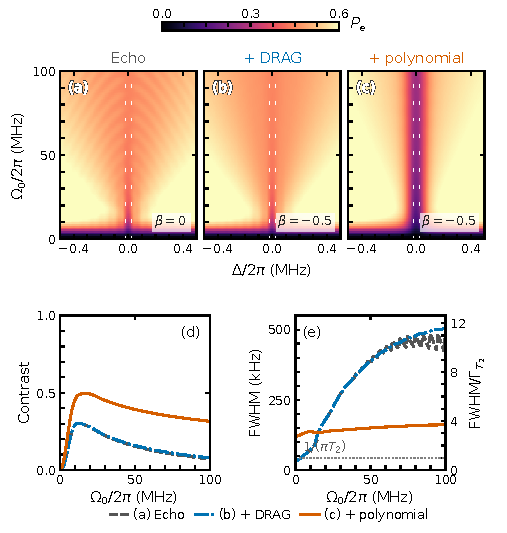
\includegraphics[width=\columnwidth]{../figures/paper/03_pulse_improvement.pdf}
    \caption{Simulated improvement through pulse shaping.
    (a)--(c) Final $P_e$ for an echo-root-Lorentzian pulse (echo),
    echo with DRAG, and echo with DRAG plus
    cutoff subtraction and a polynomial window, respectively.
    All pulses have duration $L=30~\mu\mathrm{s}$ and cutoff $c=0.001$.
    White dashed lines bracket the coherence-limited linewidth.
    (d) Resonance-center detuning. (e) Dip FWHM.
    (f) Contrast $C$, the dip depth in excited-state probability.
    DRAG compensates drive-induced detuning, suppressing resonance motion
    as the amplitude varies. The polynomial correction smooths the pulse
    edges, reducing high-drive broadening and preserving greater dip contrast.
    Together, these corrections keep the resonance more stable and
    distinguishable over a broad drive-amplitude range.}
    \label{fig:pulse-improvement}
\end{figure}
